% Lecture 1 slides
% Build with: pdflatex slides.tex (run twice)
\documentclass[aspectratio=169,11pt]{beamer}
\usepackage[T1]{fontenc}
\usepackage[utf8]{inputenc}
\usepackage{lmodern}
\usepackage{amsmath}
\usepackage{booktabs}
\usepackage{tikz}
\usetikzlibrary{arrows.meta,calc,positioning,shapes.geometric}

\definecolor{Ink}{HTML}{172033}
\definecolor{Muted}{HTML}{667085}
\definecolor{Paper}{HTML}{F7F8FC}
\definecolor{Blue}{HTML}{356AE6}
\definecolor{BlueLight}{HTML}{E9F0FF}
\definecolor{Teal}{HTML}{0E9F8A}
\definecolor{TealLight}{HTML}{DFF7F2}
\definecolor{Orange}{HTML}{F28C28}
\definecolor{OrangeLight}{HTML}{FFF0DF}
\definecolor{Red}{HTML}{D64545}
\definecolor{RedLight}{HTML}{FCE8E8}
\definecolor{Green}{HTML}{2E9B5F}
\definecolor{GreenLight}{HTML}{E4F5EB}

\setbeamercolor{normal text}{fg=Ink,bg=white}
\setbeamercolor{frametitle}{fg=Ink,bg=white}
\setbeamercolor{structure}{fg=Blue}
\setbeamercolor{block title}{fg=white,bg=Blue}
\setbeamercolor{block body}{fg=Ink,bg=BlueLight}
\setbeamercolor{itemize item}{fg=Blue}
\setbeamercolor{itemize subitem}{fg=Teal}
\setbeamertemplate{navigation symbols}{}
\setbeamertemplate{itemize item}{\raise0.15ex\hbox{\small$\bullet$}}
\setbeamertemplate{frametitle}{\vspace{0.25cm}\hspace{0.15cm}\insertframetitle\par\vspace{-0.15cm}\hspace{0.15cm}{\color{Blue}\rule{1.15cm}{2.2pt}}}
\setbeamertemplate{footline}{\leavevmode\hbox{\begin{beamercolorbox}[wd=.78\paperwidth,ht=2.8ex,dp=1.2ex,leftskip=.6cm]{normal text}\color{Muted}\scriptsize MACHINE LEARNING FROM SCRATCH \hspace{.5em}|\hspace{.5em} LECTURE 1\end{beamercolorbox}\begin{beamercolorbox}[wd=.22\paperwidth,ht=2.8ex,dp=1.2ex,rightskip=.6cm plus1fil]{normal text}\hfill\color{Muted}\scriptsize\insertframenumber\end{beamercolorbox}}}
\setbeamerfont{title}{size=\fontsize{27}{31}\selectfont,series=\bfseries}
\setbeamerfont{subtitle}{size=\large}
\setbeamerfont{frametitle}{size=\LARGE,series=\bfseries}
\setbeamerfont{block title}{series=\bfseries}

\newcommand{\key}[1]{\textcolor{Blue}{\textbf{#1}}}
\newcommand{\good}[1]{\textcolor{Green}{\textbf{#1}}}
\newcommand{\bad}[1]{\textcolor{Red}{\textbf{#1}}}
\newcommand{\pill}[2]{\tikz[baseline=(x.base)]\node[rounded corners=4pt,fill=#1,inner xsep=6pt,inner ysep=2.5pt] (x) {\scriptsize\bfseries #2};}
\newcommand{\question}[1]{\begin{center}\begin{tikzpicture}\node[rounded corners=8pt,fill=OrangeLight,draw=Orange,line width=.8pt,text width=.74\linewidth,inner sep=10pt,align=center] {\large\bfseries #1};\end{tikzpicture}\end{center}}
\newcommand{\takeaway}[1]{\begin{tikzpicture}\node[rounded corners=5pt,fill=BlueLight,text width=.82\linewidth,inner xsep=9pt,inner ysep=6pt,align=left] {\textcolor{Blue}{\textbf{Takeaway:}} #1};\end{tikzpicture}}
\tikzset{box/.style={rounded corners=5pt,draw=Blue,fill=BlueLight,thick,minimum height=1cm,align=center,inner xsep=8pt},data/.style={rounded corners=5pt,draw=Teal,fill=TealLight,thick,minimum height=1cm,align=center,inner xsep=8pt},decision/.style={diamond,aspect=2.1,draw=Orange,fill=OrangeLight,thick,align=center,inner sep=3pt},flow/.style={-{Latex[length=3mm]},thick,draw=Muted},point/.style={circle,fill=Blue,draw=white,line width=.5pt,minimum size=5pt,inner sep=0pt}}

\title{Learning from Examples}
\subtitle{From the perceptron to honest evaluation}
\author{Lecture 1}
\date{}
\begin{document}

% ================================================================
% Opening: state the problem before introducing any application
% ================================================================
\begin{frame}[plain]
  \begin{tikzpicture}[remember picture,overlay]
    \fill[Paper] (current page.south west) rectangle (current page.north east);
    \fill[Blue] (current page.north east) rectangle ([xshift=-1.25cm]current page.south east);
    \fill[Teal] ([xshift=-1.25cm]current page.north east) rectangle ([xshift=-1.65cm]current page.south east);
    \draw[Blue!18,line width=25pt] ([xshift=-2.7cm,yshift=-1.1cm]current page.north east) circle (1.25cm);
  \end{tikzpicture}
  \vspace{1.1cm}
  {\color{Blue}\small\bfseries MACHINE LEARNING FROM SCRATCH}\par\vspace{.35cm}
  {\usebeamerfont{title}\inserttitle}\par\vspace{.2cm}
  {\usebeamerfont{subtitle}\color{Muted}\insertsubtitle}\par\vspace{1cm}
  {\color{Muted}\normalsize Lecture 1}
\end{frame}

\begin{frame}{The central question}
  \begin{columns}[T,onlytextwidth]
    \column{.46\textwidth}
      \vspace{.25cm}
      A program can follow rules that we write.
      \vspace{.55cm}
      \begin{block}{Machine learning asks something different}
        Can the program discover a useful rule from labeled examples?
      \end{block}
    \column{.50\textwidth}
      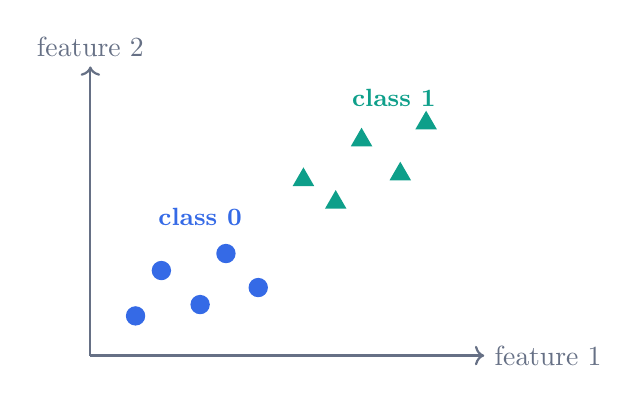
\begin{tikzpicture}[x=.82cm,y=.72cm]
        \draw[->,thick,Muted] (0,0)--(6.1,0) node[right]{feature 1};
        \draw[->,thick,Muted] (0,0)--(0,5.1) node[above]{feature 2};
        \foreach \x/\y in {.7/.7,1.1/1.5,1.7/.9,2.1/1.8,2.6/1.2}
          \node[circle,fill=Blue,minimum size=7pt,inner sep=0pt] at (\x,\y){};
        \foreach \x/\y in {3.3/3.1,3.8/2.7,4.2/3.8,4.8/3.2,5.2/4.1}
          \node[regular polygon,regular polygon sides=3,fill=Teal,minimum size=9pt,inner sep=0pt] at (\x,\y){};
        \node[Blue,font=\small\bfseries] at (1.7,2.45){class 0};
        \node[Teal,font=\small\bfseries] at (4.7,4.55){class 1};
      \end{tikzpicture}
  \end{columns}
  \vspace{.15cm}\question{Where should a new point belong?}
\end{frame}

\begin{frame}{Today's chain of ideas}
  \begin{center}
    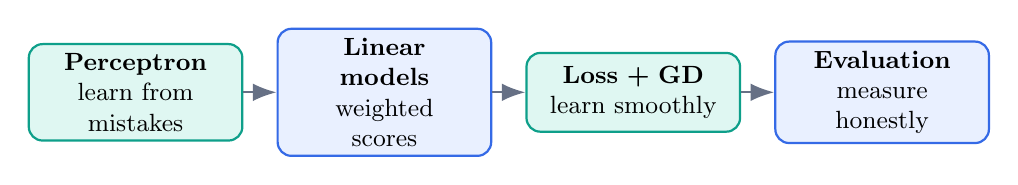
\begin{tikzpicture}[node distance=.42cm,every node/.style={font=\small}]
      \node[data,text width=2.15cm](a){\textbf{Perceptron}\\learn from mistakes};
      \node[box,text width=2.15cm,right=of a](b){\textbf{Linear models}\\weighted scores};
      \node[data,text width=2.15cm,right=of b](c){\textbf{Loss + GD}\\learn smoothly};
      \node[box,text width=2.15cm,right=of c](d){\textbf{Evaluation}\\measure honestly};
      \draw[flow](a)--(b);\draw[flow](b)--(c);\draw[flow](c)--(d);
    \end{tikzpicture}
  \end{center}
  \vspace{.75cm}
  \begin{itemize}
    \item Begin with the simplest trainable classifier
    \item Reuse its weighted score for regression and probabilities
    \item End by asking whether the learned rule will generalize
  \end{itemize}
\end{frame}

% ================================================================
% Perceptron: the first complete learning algorithm
% ================================================================
\section{Perceptron}

\begin{frame}{Start with a straight decision boundary}
  \begin{columns}[T,onlytextwidth]
    \column{.57\textwidth}
      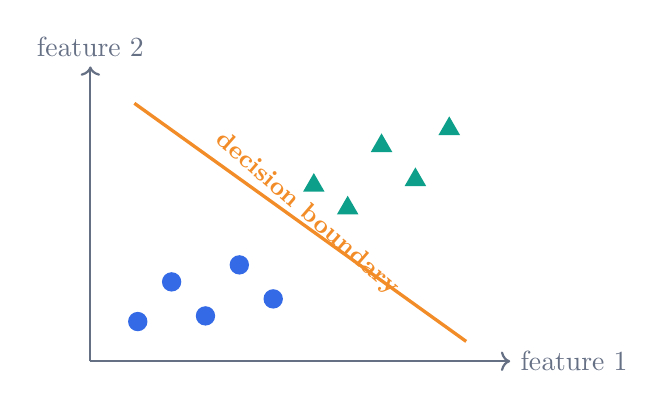
\begin{tikzpicture}[x=.86cm,y=.72cm]
        \draw[->,thick,Muted] (0,0)--(6.2,0) node[right]{feature 1};
        \draw[->,thick,Muted] (0,0)--(0,5.2) node[above]{feature 2};
        \foreach \x/\y in {.7/.7,1.2/1.4,1.7/.8,2.2/1.7,2.7/1.1}
          \node[circle,fill=Blue,minimum size=7pt,inner sep=0pt] at (\x,\y){};
        \foreach \x/\y in {3.3/3.1,3.8/2.7,4.3/3.8,4.8/3.2,5.3/4.1}
          \node[regular polygon,regular polygon sides=3,fill=Teal,minimum size=9pt,inner sep=0pt] at (\x,\y){};
        \draw[very thick,Orange] (.65,4.55)--(5.55,.35);
        \node[rotate=-41,Orange,font=\small\bfseries] at (3.2,2.6){decision boundary};
      \end{tikzpicture}
    \column{.39\textwidth}
      \vspace{.45cm}
      \begin{itemize}
        \item One side predicts class 0
        \item The other predicts class 1
        \item Training moves the boundary
      \end{itemize}
  \end{columns}
  \vspace{.1cm}\takeaway{A perceptron is a trainable linear classifier.}
\end{frame}

\begin{frame}{The boundary comes from a weighted score}
  \begin{center}
    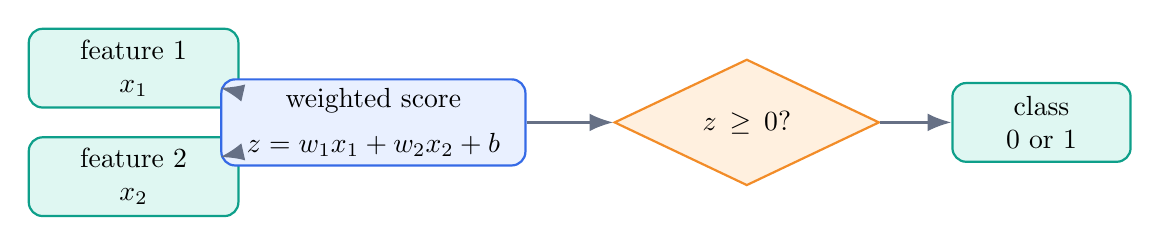
\begin{tikzpicture}[node distance=.7cm]
      \node[data,text width=2.1cm](x1){feature 1\\$x_1$};
      \node[data,text width=2.1cm,below=.35cm of x1](x2){feature 2\\$x_2$};
      \node[box,text width=3.3cm,right=1.1cm of $(x1)!0.5!(x2)$](score){weighted score\\[4pt]$z=w_1x_1+w_2x_2+b$};
      \node[decision,right=1.1cm of score,text width=2.1cm](check){$z\geq 0$?};
      \node[data,right=.9cm of check,text width=1.7cm](out){class\\0 or 1};
      \draw[flow](x1)--(score);\draw[flow](x2)--(score);\draw[flow](score)--(check);\draw[flow](check)--(out);
    \end{tikzpicture}
  \end{center}
  \vspace{.55cm}
  \begin{itemize}
    \item Weights control the boundary's direction
    \item The bias moves the boundary without rotating it
  \end{itemize}
\end{frame}

\begin{frame}{A score becomes a hard decision}
  \begin{center}
    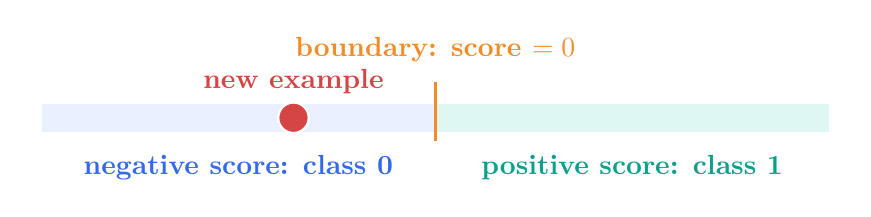
\begin{tikzpicture}[x=10cm,y=1cm]
      \draw[line width=10pt,BlueLight] (0,0)--(.5,0);
      \draw[line width=10pt,TealLight] (.5,0)--(1,0);
      \draw[very thick,Orange] (.5,-.3)--(.5,.45);
      \node[above=4pt,Orange,font=\bfseries] at (.5,.45){boundary: score $=0$};
      \node[below=10pt,Blue,font=\bfseries] at (.25,0){negative score: class 0};
      \node[below=10pt,Teal,font=\bfseries] at (.75,0){positive score: class 1};
      \node[circle,fill=Red,draw=white,thick,minimum size=11pt] at (.32,0){};
      \node[above=5pt,Red,font=\bfseries] at (.32,0){new example};
    \end{tikzpicture}
  \end{center}
  \vspace{1cm}\takeaway{Prediction is easy once the weights and bias are known. Learning them is the interesting part.}
\end{frame}

\begin{frame}{The perceptron learns from mistakes}
  \begin{center}
    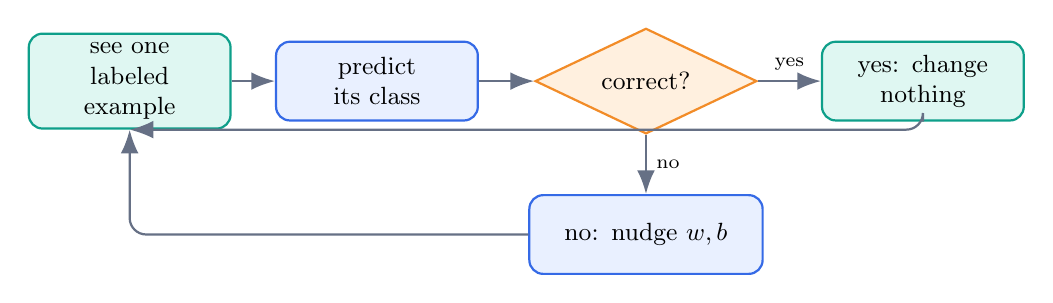
\begin{tikzpicture}[node distance=.55cm,every node/.style={font=\small}]
      \node[data,text width=2cm](see){see one labeled example};
      \node[box,text width=2cm,right=of see](predict){predict its class};
      \node[decision,right=.7cm of predict,text width=1.7cm](correct){correct?};
      \node[data,right=.8cm of correct,text width=2cm](keep){yes: change nothing};
      \node[box,below=.75cm of correct,text width=2.4cm](move){no: nudge $w,b$};
      \draw[flow](see)--(predict);\draw[flow](predict)--(correct);
      \draw[flow](correct)--node[above,font=\scriptsize]{yes}(keep);
      \draw[flow](correct)--node[right,font=\scriptsize]{no}(move);
      \draw[flow,rounded corners=6pt](keep.south)|-(see.south);
      \draw[flow,rounded corners=6pt](move.west)-|(see.south);
    \end{tikzpicture}
  \end{center}
  \vspace{.5cm}
  \begin{block}{Mistake-driven rule}
    Correct examples make no update. Wrong examples move the boundary toward a better decision.
  \end{block}
\end{frame}

\begin{frame}{What does one update try to do?}
  \begin{columns}[T,onlytextwidth]
    \column{.52\textwidth}
      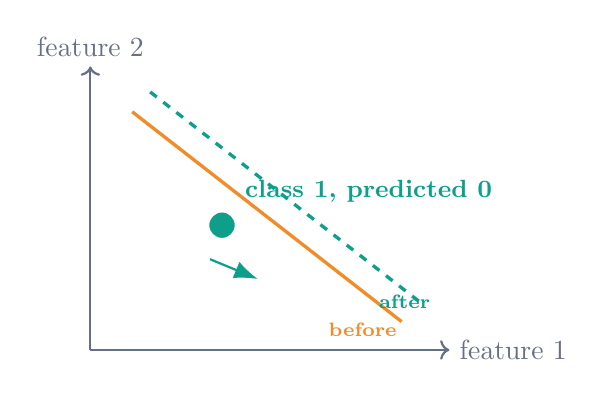
\begin{tikzpicture}[x=.76cm,y=.72cm]
        \draw[->,thick,Muted](0,0)--(6,0)node[right]{feature 1};
        \draw[->,thick,Muted](0,0)--(0,5)node[above]{feature 2};
        \draw[very thick,Orange](.7,4.2)--(5.2,.5);
        \draw[very thick,Teal,dashed](1.0,4.55)--(5.5,.85);
        \node[circle,fill=Teal,draw=white,thick,minimum size=10pt] (miss) at (2.2,2.2){};
        \node[Teal,font=\small\bfseries,above right=.05cm of miss]{class 1, predicted 0};
        \draw[flow,Teal](2.0,1.6)--(2.8,1.25);
        \node[Orange,font=\scriptsize\bfseries]at(4.55,.35){before};
        \node[Teal,font=\scriptsize\bfseries]at(5.25,.85){after};
      \end{tikzpicture}
    \column{.44\textwidth}
      \begin{itemize}
        \item Increase the example's score if its true class is 1
        \item Decrease the score if its true class is 0
        \item Repeat over the data for several passes
      \end{itemize}
  \end{columns}
\end{frame}

\begin{frame}{The perceptron is powerful---and limited}
  \begin{columns}[T,onlytextwidth]
    \column{.47\textwidth}
      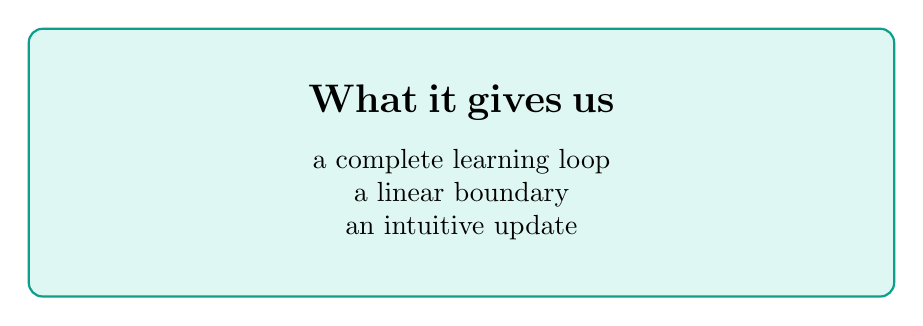
\begin{tikzpicture}\node[data,text width=.86\linewidth,minimum height=3.4cm]{
        {\Large\bfseries What it gives us}\\[8pt]
        a complete learning loop\\a linear boundary\\an intuitive update
      };\end{tikzpicture}
    \column{.47\textwidth}
      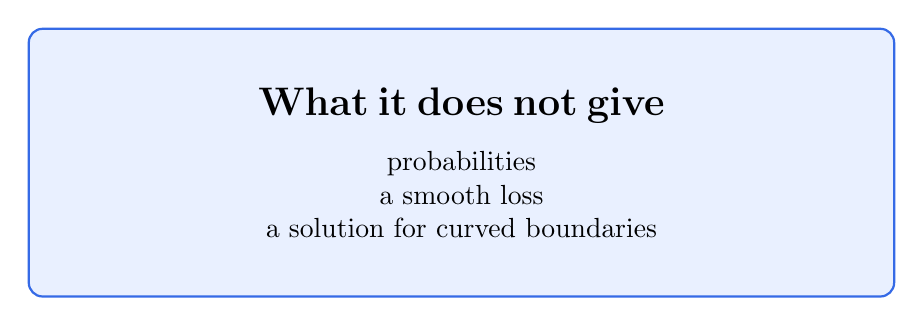
\begin{tikzpicture}\node[box,text width=.86\linewidth,minimum height=3.4cm]{
        {\Large\bfseries What it does not give}\\[8pt]
        probabilities\\a smooth loss\\a solution for curved boundaries
      };\end{tikzpicture}
  \end{columns}
  \vspace{.4cm}\question{How can we keep the weighted score but obtain richer outputs and smoother learning?}
\end{frame}

% ================================================================
% One linear score, then regression and gradient descent
% ================================================================
\section{Linear models and learning}

\begin{frame}{One score, three interpretations}
  \begin{center}
    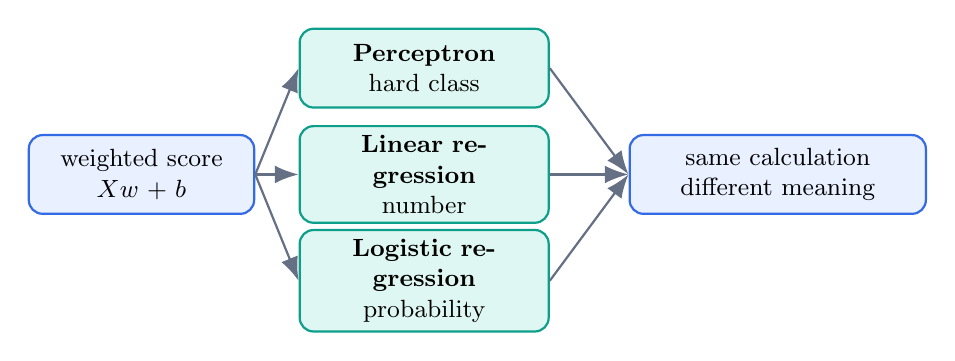
\begin{tikzpicture}[node distance=.55cm,every node/.style={font=\small}]
      \node[box,text width=2.3cm](score){weighted score\\$Xw+b$};
      \node[data,text width=2.6cm,right=of score,yshift=1.35cm](p){\textbf{Perceptron}\\hard class};
      \node[data,text width=2.6cm,right=of score](lin){\textbf{Linear regression}\\number};
      \node[data,text width=2.6cm,right=of score,yshift=-1.35cm](log){\textbf{Logistic regression}\\probability};
      \draw[flow](score.east)--(p.west);\draw[flow](score.east)--(lin.west);\draw[flow](score.east)--(log.west);
      \node[box,text width=3.2cm,right=1cm of lin](meaning){same calculation\\different meaning};
      \draw[flow](p.east)--(meaning.west);\draw[flow](lin.east)--(meaning.west);\draw[flow](log.east)--(meaning.west);
    \end{tikzpicture}
  \end{center}
  \vspace{.35cm}\takeaway{The output meaning determines the activation, loss, and evaluation metric.}
\end{frame}

\begin{frame}{Linear regression predicts a number}
  \begin{columns}[T,onlytextwidth]
    \column{.60\textwidth}
      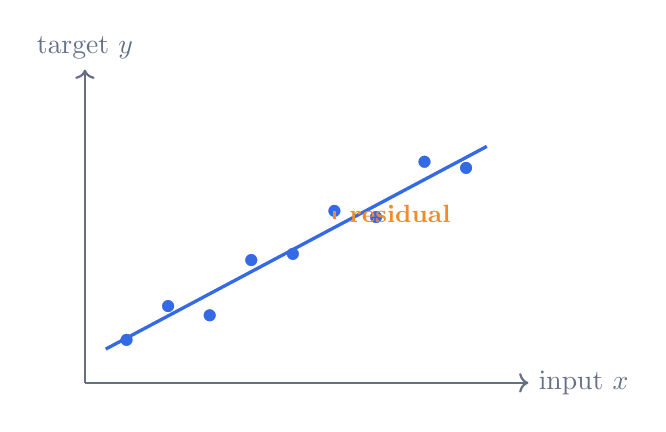
\begin{tikzpicture}[x=.88cm,y=.78cm]
        \draw[->,thick,Muted](0,0)--(6.4,0)node[right]{input $x$};
        \draw[->,thick,Muted](0,0)--(0,5.1)node[above]{target $y$};
        \foreach \x/\y in {.6/.7,1.2/1.25,1.8/1.1,2.4/2,3/2.1,3.6/2.8,4.2/2.7,4.9/3.6,5.5/3.5}\node[point]at(\x,\y){};
        \draw[very thick,Blue](.3,.55)--(5.8,3.85);
        \draw[dashed,Orange,thick](3.6,2.8)--(3.6,2.53);
        \node[Orange,font=\small\bfseries,anchor=west]at(3.68,2.75){residual};
      \end{tikzpicture}
    \column{.36\textwidth}
      \vspace{.35cm}
      \[\hat y=wx+b\]
      \begin{itemize}
        \item $w$: slope
        \item $b$: vertical offset
        \item residual: prediction minus answer
      \end{itemize}
  \end{columns}
\end{frame}

\begin{frame}{A loss defines what ``better'' means}
  \begin{columns}[T,onlytextwidth]
    \column{.51\textwidth}
      \begin{itemize}
        \item A model makes many residuals
        \item We need one number to compare parameter choices
        \item The loss becomes the training objective
      \end{itemize}
      \vspace{.35cm}
      \begin{block}{Mean-squared error (MSE)}
        Square each residual, then average.
        \[\text{MSE}=\text{average}\big((\hat y-y)^2\big)\]
      \end{block}
    \column{.45\textwidth}
      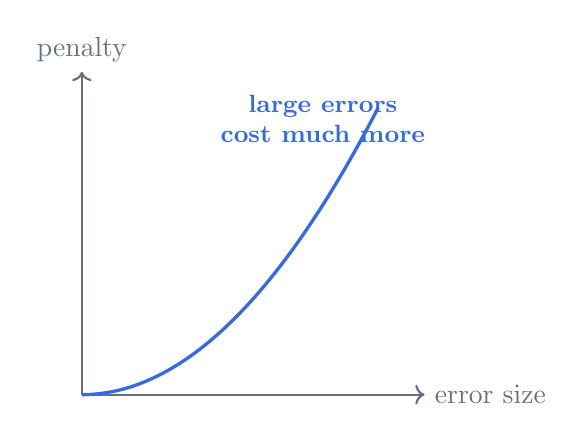
\begin{tikzpicture}[x=.68cm,y=.5cm]
        \draw[->,thick,Muted](0,0)--(6.4,0)node[right]{error size};
        \draw[->,thick,Muted](0,0)--(0,8.2)node[above]{penalty};
        \draw[very thick,Blue,domain=0:2.7,samples=50,smooth]plot({2.05*\x},{\x*\x});
        \node[Blue,font=\small\bfseries,align=center]at(4.5,7.0){large errors\\cost much more};
      \end{tikzpicture}
  \end{columns}
\end{frame}

\begin{frame}{Now learning has a direction}
  \begin{center}
    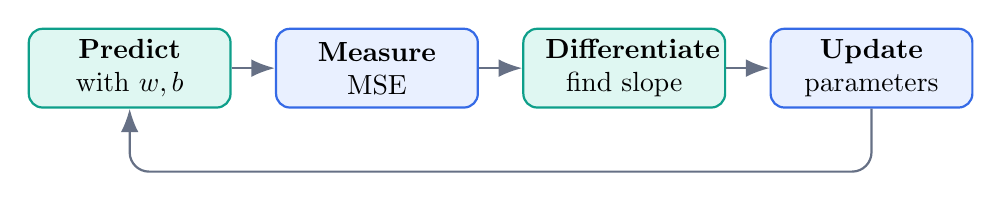
\begin{tikzpicture}[node distance=.55cm]
      \node[data,text width=2cm](predict){\textbf{Predict}\\with $w,b$};
      \node[box,text width=2cm,right=of predict](measure){\textbf{Measure}\\MSE};
      \node[data,text width=2cm,right=of measure](gradient){\textbf{Differentiate}\\find slope};
      \node[box,text width=2cm,right=of gradient](update){\textbf{Update}\\parameters};
      \draw[flow](predict)--(measure);\draw[flow](measure)--(gradient);\draw[flow](gradient)--(update);
      \draw[flow,rounded corners=7pt](update.south)--++(0,-.8)-|(predict.south);
    \end{tikzpicture}
  \end{center}
  \vspace{.65cm}\takeaway{Gradient descent replaces mistake-by-mistake jumps with small steps that reduce a smooth loss.}
\end{frame}

\begin{frame}{A gradient is a downhill signpost}
  \begin{columns}[T,onlytextwidth]
    \column{.58\textwidth}
      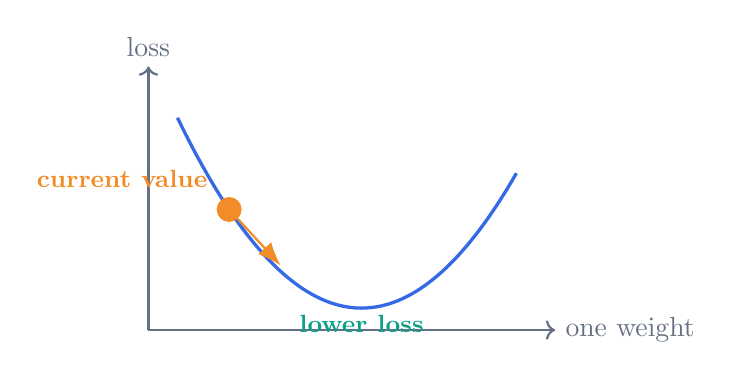
\begin{tikzpicture}[x=.82cm,y=.62cm]
        \draw[->,thick,Muted](0,0)--(6.3,0)node[right]{one weight};
        \draw[->,thick,Muted](0,0)--(0,5.4)node[above]{loss};
        \draw[very thick,Blue,domain=.45:5.7,samples=60,smooth]plot(\x,{.48*(\x-3.3)*(\x-3.3)+.45});
        \node[circle,fill=Orange,minimum size=9pt,inner sep=0pt](now)at(1.25,2.47){};
        \draw[flow,Orange](now)--(2.05,1.32);
        \node[Orange,font=\small\bfseries,above left=.05cm of now]{current value};
        \node[Teal,font=\small\bfseries]at(3.3,.12){lower loss};
      \end{tikzpicture}
    \column{.38\textwidth}
      \vspace{.45cm}
      {\small\begin{align*}
        \text{new value}={}&\text{old value}\\[-2pt]
        &-\eta\times\text{gradient}
      \end{align*}}
      $\eta$ is the \key{learning rate}: the step size.
  \end{columns}
\end{frame}

\begin{frame}{The learning rate controls convergence}
  \begin{columns}[T,onlytextwidth]
    \column{.31\textwidth}\begin{tikzpicture}\node[rounded corners=6pt,fill=BlueLight,text width=.82\linewidth,minimum height=4cm,align=center]{\textbf{Too small}\\[8pt]\begin{tikzpicture}[x=.42cm,y=.35cm]\draw[thick,Blue]plot[smooth]coordinates{(0,3)(1,2.7)(2,2.45)(3,2.2)(4,2)(5,1.85)};\end{tikzpicture}\\[7pt]safe, but slow};\end{tikzpicture}
    \column{.31\textwidth}\begin{tikzpicture}\node[rounded corners=6pt,fill=TealLight,text width=.82\linewidth,minimum height=4cm,align=center]{\textbf{Useful}\\[8pt]\begin{tikzpicture}[x=.42cm,y=.35cm]\draw[thick,Teal]plot[smooth]coordinates{(0,3)(1,1.5)(2,.75)(3,.45)(4,.34)(5,.31)};\end{tikzpicture}\\[7pt]steady convergence};\end{tikzpicture}
    \column{.31\textwidth}\begin{tikzpicture}\node[rounded corners=6pt,fill=RedLight,text width=.82\linewidth,minimum height=4cm,align=center]{\textbf{Too large}\\[8pt]\begin{tikzpicture}[x=.42cm,y=.35cm]\draw[thick,Red]plot coordinates{(0,2.4)(1,.8)(2,2.7)(3,.45)(4,3.2)(5,.2)};\end{tikzpicture}\\[7pt]jumps or diverges};\end{tikzpicture}
  \end{columns}
\end{frame}

\begin{frame}{Convergence is not the same as generalization}
  \begin{columns}[T,onlytextwidth]
    \column{.55\textwidth}
      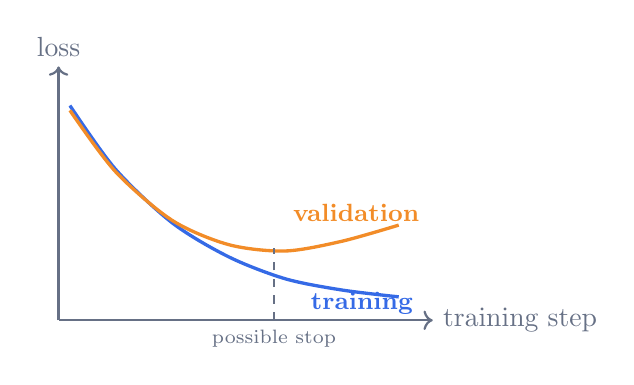
\begin{tikzpicture}[x=.72cm,y=.62cm]
        \draw[->,thick,Muted](0,0)--(6.6,0)node[right]{training step};
        \draw[->,thick,Muted](0,0)--(0,5.2)node[above]{loss};
        \draw[very thick,Blue]plot[smooth]coordinates{(.2,4.4)(1,3.1)(2,2)(3,1.3)(4,.85)(5,.62)(6,.48)};
        \draw[very thick,Orange]plot[smooth]coordinates{(.2,4.3)(1,3.05)(2,2.05)(3,1.55)(4,1.42)(5,1.62)(6,1.95)};
        \node[Blue,font=\small\bfseries]at(5.35,.35){training};
        \node[Orange,font=\small\bfseries]at(5.25,2.2){validation};
        \draw[dashed,Muted](3.8,0)--(3.8,1.48);
        \node[below,Muted,font=\scriptsize]at(3.8,0){possible stop};
      \end{tikzpicture}
    \column{.41\textwidth}
      \begin{itemize}
        \item Training loss: fit to seen examples
        \item Validation loss: behavior on unseen examples
        \item A growing gap suggests overfitting
      \end{itemize}
  \end{columns}
\end{frame}

% ================================================================
% Logistic regression: smooth probabilities built on the same score
% ================================================================
\section{Logistic regression}

\begin{frame}{A hard score cannot express uncertainty}
  \begin{center}
    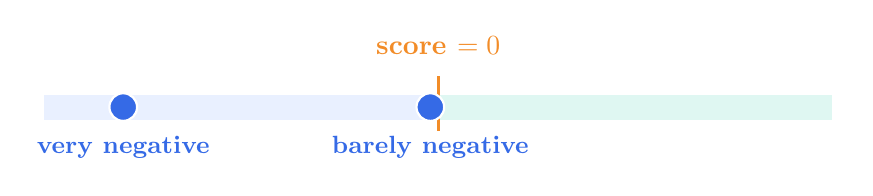
\begin{tikzpicture}[x=10cm,y=1cm]
      \draw[line width=9pt,BlueLight](0,0)--(.5,0);
      \draw[line width=9pt,TealLight](.5,0)--(1,0);
      \draw[very thick,Orange](.5,-.3)--(.5,.4);
      \node[above=4pt,Orange,font=\bfseries]at(.5,.4){score $=0$};
      \node[circle,fill=Blue,draw=white,thick,minimum size=10pt]at(.1,0){};
      \node[circle,fill=Blue,draw=white,thick,minimum size=10pt]at(.49,0){};
      \node[below=7pt,Blue,font=\small\bfseries]at(.1,0){very negative};
      \node[below=7pt,Blue,font=\small\bfseries]at(.49,0){barely negative};
    \end{tikzpicture}
  \end{center}
  \vspace{.85cm}
  The perceptron calls both points class 0, but they should not express the same confidence.
  \vspace{.45cm}
  \question{Can we turn distance from the boundary into a smooth value between 0 and 1?}
\end{frame}

\begin{frame}{The sigmoid turns score into probability}
  \begin{columns}[T,onlytextwidth]
    \column{.63\textwidth}
      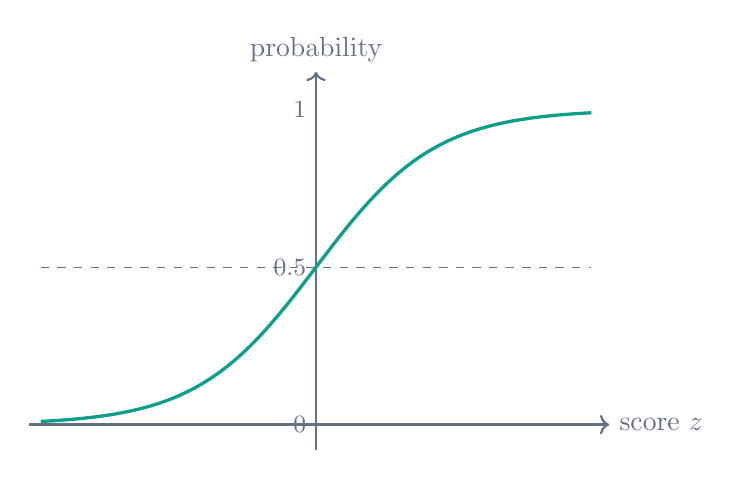
\begin{tikzpicture}[x=.76cm,y=4cm]
        \draw[->,thick,Muted](-4.8,0)--(4.9,0)node[right]{score $z$};
        \draw[->,thick,Muted](0,-.08)--(0,1.12)node[above]{probability};
        \draw[dashed,Muted](-4.6,.5)--(4.6,.5);
        \draw[very thick,Teal,domain=-4.6:4.6,samples=80,smooth]plot(\x,{1/(1+exp(-\x))});
        \node[left,Muted,font=\small]at(0,0){$0$};
        \node[left,Muted,font=\small]at(0,.5){$0.5$};
        \node[left,Muted,font=\small]at(0,1){$1$};
      \end{tikzpicture}
    \column{.33\textwidth}
      \vspace{.7cm}
      \[p=\sigma(z)=\frac{1}{1+e^{-z}}\]
      \begin{itemize}
        \item smooth
        \item bounded
        \item differentiable
      \end{itemize}
  \end{columns}
\end{frame}

\begin{frame}{Activation and loss solve different problems}
  \begin{columns}[T,onlytextwidth]
    \column{.47\textwidth}
      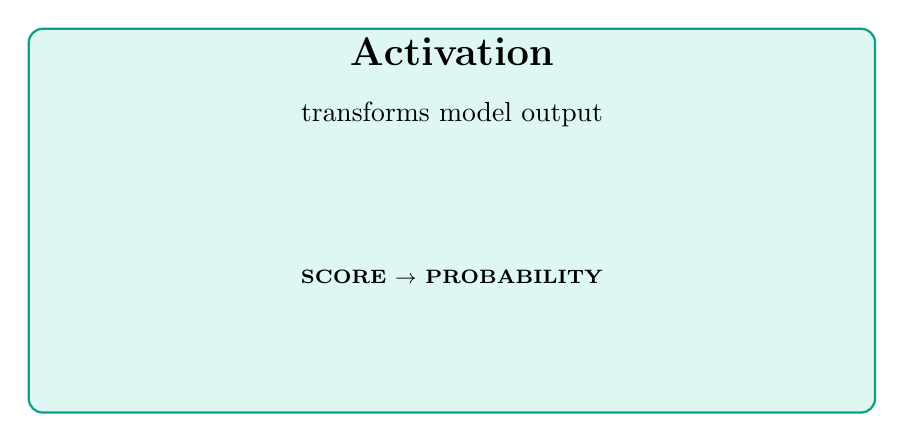
\begin{tikzpicture}\node[data,text width=.84\linewidth,minimum height=3.2cm]{
        {\Large\bfseries Activation}\\[8pt]
        transforms model output\\[8pt]
        \pill{TealLight}{SCORE $\rightarrow$ PROBABILITY}
      };\end{tikzpicture}
    \column{.47\textwidth}
      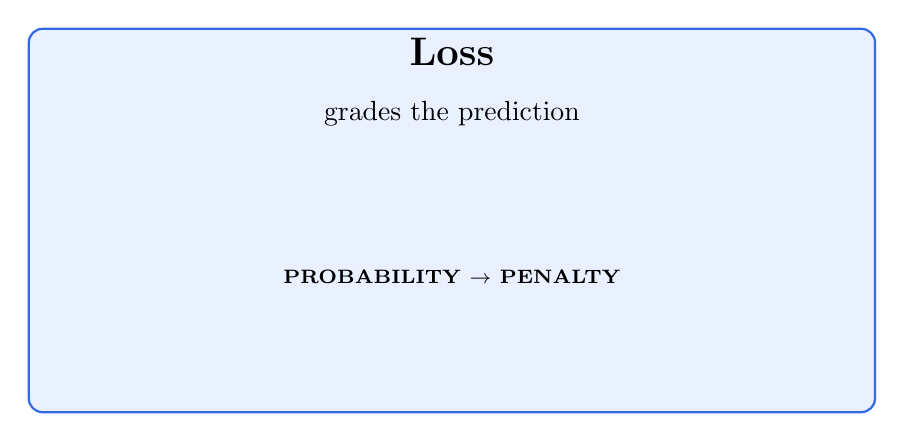
\begin{tikzpicture}\node[box,text width=.84\linewidth,minimum height=3.2cm]{
        {\Large\bfseries Loss}\\[8pt]
        grades the prediction\\[8pt]
        \pill{BlueLight}{PROBABILITY $\rightarrow$ PENALTY}
      };\end{tikzpicture}
  \end{columns}
  \vspace{.45cm}\takeaway{For logistic regression, sigmoid is the activation and binary cross-entropy is the loss.}
\end{frame}

\begin{frame}{Binary cross-entropy cares about confidence}
  \begin{columns}[T,onlytextwidth]
    \column{.50\textwidth}
      \begin{block}{Suppose the true class is 1}
        Predict $0.9$: small penalty\\
        Predict $0.6$: moderate penalty\\
        Predict $0.1$: very large penalty
      \end{block}
      \vspace{.3cm}
      \begin{itemize}
        \item Correct and confident is rewarded
        \item Wrong and confident is punished strongly
        \item Smooth changes give useful gradients
      \end{itemize}
    \column{.46\textwidth}
      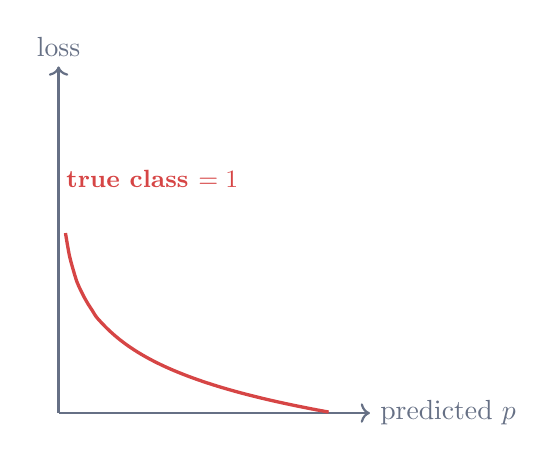
\begin{tikzpicture}[x=3.5cm,y=.62cm]
        \draw[->,thick,Muted](0,0)--(1.13,0)node[right]{predicted $p$};
        \draw[->,thick,Muted](0,0)--(0,7.1)node[above]{loss};
        \draw[very thick,Red,domain=.025:.98,samples=70,smooth]plot(\x,{-ln(\x)});
        \node[Red,font=\small\bfseries]at(.34,4.8){true class $=1$};
      \end{tikzpicture}
  \end{columns}
\end{frame}

\begin{frame}{Why not use accuracy as the training loss?}
  \begin{center}
    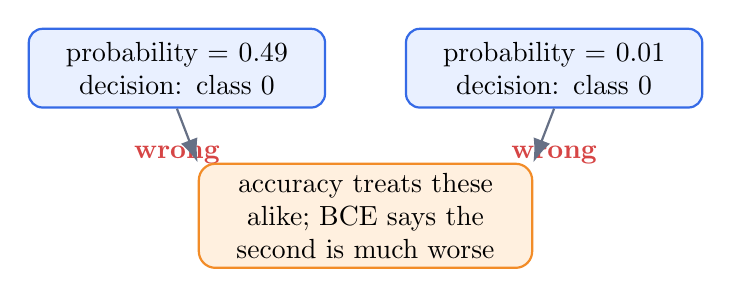
\begin{tikzpicture}[node distance=1cm]
      \node[box,text width=3.2cm](a){probability $=0.49$\\decision: class 0};
      \node[box,text width=3.2cm,right=of a](b){probability $=0.01$\\decision: class 0};
      \node[below=.35cm of a,Red,font=\bfseries]{wrong};
      \node[below=.35cm of b,Red,font=\bfseries]{wrong};
      \node[rounded corners=6pt,fill=OrangeLight,draw=Orange,thick,text width=4cm,align=center,below=1.2cm of $(a)!0.5!(b)$](loss){accuracy treats these alike; BCE says the second is much worse};
      \draw[flow](a.south)--(loss.north west);\draw[flow](b.south)--(loss.north east);
    \end{tikzpicture}
  \end{center}
  \vspace{.25cm}\takeaway{A training loss must show how to improve before the hard decision flips.}
\end{frame}

\begin{frame}{Logistic regression reuses gradient descent}
  \begin{center}
    \resizebox{.94\textwidth}{!}{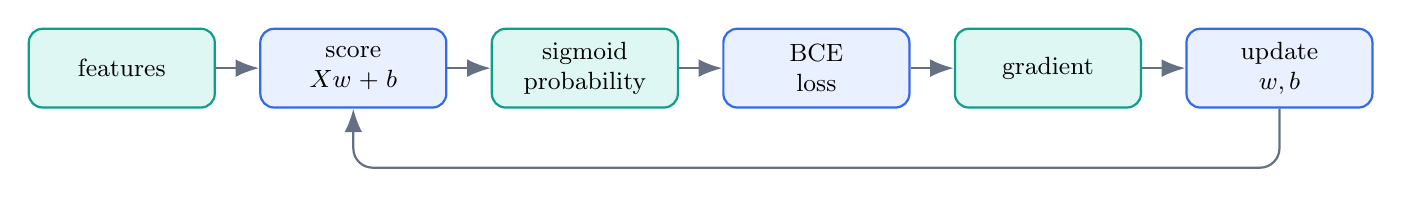
\begin{tikzpicture}[node distance=.55cm,every node/.style={font=\small}]
      \node[data,text width=1.8cm](x){features};
      \node[box,text width=1.8cm,right=of x](z){score\\$Xw+b$};
      \node[data,text width=1.8cm,right=of z](p){sigmoid\\probability};
      \node[box,text width=1.8cm,right=of p](l){BCE\\loss};
      \node[data,text width=1.8cm,right=of l](g){gradient};
      \node[box,text width=1.8cm,right=of g](u){update\\$w,b$};
      \draw[flow](x)--(z);\draw[flow](z)--(p);\draw[flow](p)--(l);\draw[flow](l)--(g);\draw[flow](g)--(u);
      \draw[flow,rounded corners=7pt](u.south)--++(0,-.75)-|(z.south);
    \end{tikzpicture}}
  \end{center}
  \vspace{.65cm}
  \begin{itemize}
    \item The model learns a smooth probability, not a final action
    \item A separate threshold later turns probability into a decision
  \end{itemize}
\end{frame}

\begin{frame}{Perceptron and logistic regression are cousins}
  \begin{center}
    \begin{tabular}{@{}lll@{}}
      \toprule
      &\textbf{Perceptron}&\textbf{Logistic regression}\\
      \midrule
      Shared core&weighted score&weighted score\\
      Output&hard class&probability\\
      Learning signal&mistakes&BCE gradient\\
      Updates&only when wrong&every non-perfect prediction\\
      Typical use&simple decisions&risk ranking / probability\\
      \bottomrule
    \end{tabular}
  \end{center}
  \vspace{.7cm}\takeaway{Same linear geometry; different output and learning signal.}
\end{frame}

% ================================================================
% Evaluation: first decisions, then metrics, then data discipline
% ================================================================
\section{Evaluation}

\begin{frame}{Probability and decision are separate}
  \begin{center}
    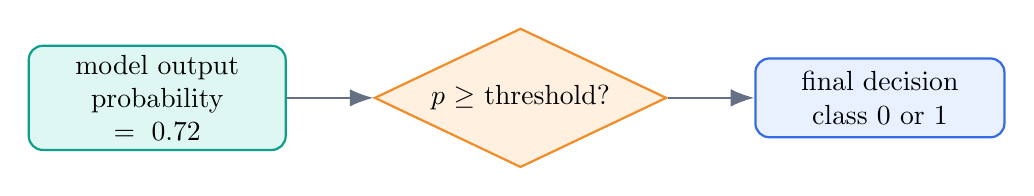
\begin{tikzpicture}[node distance=.8cm]
      \node[data,text width=2.7cm](model){model output\\probability $=0.72$};
      \node[decision,right=1.1cm of model,text width=2.4cm](compare){$p\geq$ threshold?};
      \node[box,right=1.1cm of compare,text width=2.6cm](action){final decision\\class 0 or 1};
      \draw[flow](model)--(compare);\draw[flow](compare)--(action);
    \end{tikzpicture}
  \end{center}
  \vspace{.65cm}
  \begin{itemize}
    \item Training learns weights that produce probabilities
    \item Validation chooses a threshold for the real decision
    \item Changing the threshold does not retrain the probability model
  \end{itemize}
\end{frame}

\begin{frame}{Every binary prediction lands in one box}
  \begin{center}
    \begin{tabular}{cc|c|c|}
      \multicolumn{2}{c}{}&\multicolumn{2}{c}{\textbf{Actual}}\\
      \multicolumn{2}{c}{}&\textbf{Positive}&\textbf{Negative}\\\cline{3-4}
      \textbf{Predicted}&\textbf{Positive}&\good{TP}: found&\textcolor{Orange}{\textbf{FP}}: false alarm\\\cline{3-4}
      &\textbf{Negative}&\bad{FN}: missed&\key{TN}: rejected\\\cline{3-4}
    \end{tabular}
  \end{center}
  \vspace{.6cm}
  \begin{itemize}
    \item Accuracy merges all four boxes into one number
    \item Precision and recall focus on different kinds of error
  \end{itemize}
\end{frame}

\begin{frame}{The accuracy trap}
  \begin{columns}[T,onlytextwidth]
    \column{.59\textwidth}
      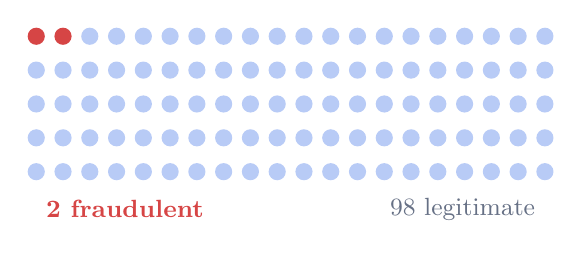
\begin{tikzpicture}[x=.34cm,y=.43cm]
        \foreach \r in {0,...,4}{\foreach \c in {0,...,19}{
          \pgfmathtruncatemacro{\idx}{20*\r+\c}
          \ifnum\idx<2\fill[Red](\c,-\r)circle(3.1pt);\else\fill[Blue!35](\c,-\r)circle(3.1pt);\fi}}
        \node[anchor=west,Red,font=\small\bfseries]at(0,-5.1){2 fraudulent};
        \node[anchor=east,Muted,font=\small]at(19,-5.1){98 legitimate};
      \end{tikzpicture}
    \column{.37\textwidth}
      \vspace{.35cm}
      Predict ``legitimate'' every time:
      \vspace{.25cm}
      \begin{center}{\fontsize{30}{34}\selectfont\bfseries\color{Blue}98\%}\\accuracy\end{center}
      \vspace{.25cm}{\color{Red}\bfseries But no fraud is found.}
  \end{columns}
  \vspace{.15cm}\takeaway{Class imbalance can make a useless classifier look excellent.}
\end{frame}

\begin{frame}{Metrics answer different questions}
  \begin{center}
    \begin{tabular}{@{}lll@{}}
      \toprule
      \textbf{Metric}&\textbf{Question}&\textbf{Formula}\\
      \midrule
      Accuracy&How often are we right?&$(TP+TN)/\text{all}$\\
      Precision&When we flag, how often right?&$TP/(TP+FP)$\\
      Recall&Of all positives, how many found?&$TP/(TP+FN)$\\
      F1&Balance precision and recall&harmonic balance\\
      F2&Favor recall more strongly&recall-weighted balance\\
      \bottomrule
    \end{tabular}
  \end{center}
  \vspace{.6cm}\takeaway{Choose a metric because it matches the task, not because it is familiar.}
\end{frame}

\begin{frame}{Precision and recall express a trade-off}
  \begin{columns}[T,onlytextwidth]
    \column{.47\textwidth}
      
\begin{tikzpicture}\node[rounded corners=6pt,fill=BlueLight,text width=.84\linewidth,minimum height=3.4cm,align=center]{
        {\Large\bfseries High precision}\\[8pt]
        few false alarms\\[5pt]
        some positives may be missed
      };\end{tikzpicture}
    \column{.47\textwidth}
      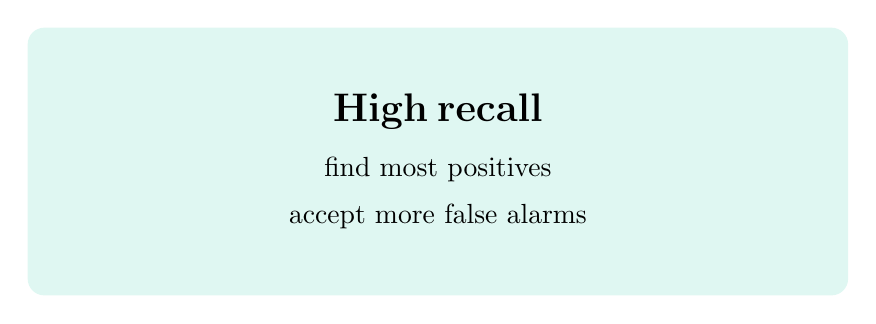
\begin{tikzpicture}\node[rounded corners=6pt,fill=TealLight,text width=.84\linewidth,minimum height=3.4cm,align=center]{
        {\Large\bfseries High recall}\\[8pt]
        find most positives\\[5pt]
        accept more false alarms
      };\end{tikzpicture}
  \end{columns}
  \vspace{.45cm}\question{Which error matters more in the application we are building?}
\end{frame}

\begin{frame}{The threshold moves the trade-off}
  \begin{center}
    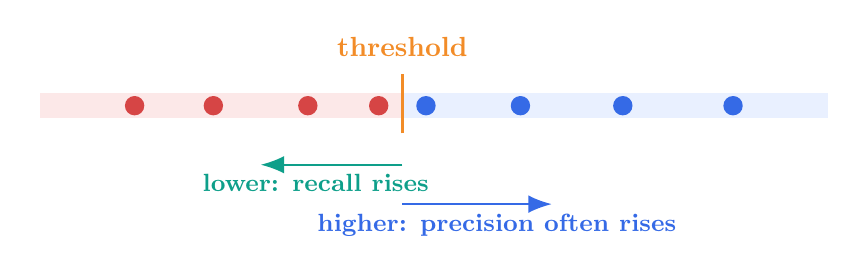
\begin{tikzpicture}[x=10cm,y=1cm]
      \draw[line width=9pt,RedLight](0,0)--(.46,0);\draw[line width=9pt,BlueLight](.46,0)--(1,0);
      \foreach \x in {.12,.22,.34,.43}\node[circle,fill=Red,minimum size=7pt,inner sep=0pt]at(\x,0){};
      \foreach \x in {.49,.61,.74,.88}\node[circle,fill=Blue,minimum size=7pt,inner sep=0pt]at(\x,0){};
      \draw[very thick,Orange](.46,-.35)--(.46,.4);\node[above=3pt,Orange,font=\bfseries]at(.46,.4){threshold};
      \draw[flow,Teal](.46,-.75)--(.28,-.75);\node[below,Teal,font=\small\bfseries]at(.35,-.75){lower: recall rises};
      \draw[flow,Blue](.46,-1.25)--(.65,-1.25);\node[below,Blue,font=\small\bfseries]at(.58,-1.25){higher: precision often rises};
    \end{tikzpicture}
  \end{center}
  \vspace{.45cm}\takeaway{There is no universally correct threshold---only a threshold chosen for a purpose.}
\end{frame}

\begin{frame}{Remove models that are worse in both ways}
  \begin{columns}[T,onlytextwidth]
    \column{.60\textwidth}
      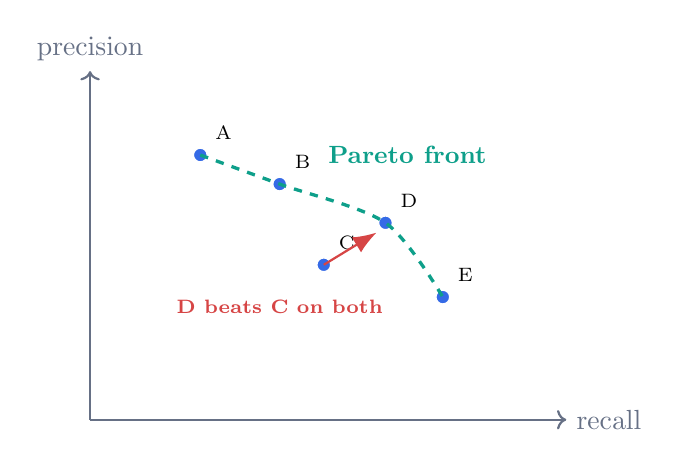
\begin{tikzpicture}[x=5.6cm,y=4.1cm]
        \draw[->,thick,Muted](0,0)--(1.08,0)node[right]{recall};
        \draw[->,thick,Muted](0,0)--(0,1.08)node[above]{precision};
        \node[point,label={[font=\scriptsize]above right:A}]at(.25,.82){};
        \node[point,label={[font=\scriptsize]above right:B}]at(.43,.73){};
        \node[point,label={[font=\scriptsize]above right:C}]at(.53,.48){};
        \node[point,label={[font=\scriptsize]above right:D}]at(.67,.61){};
        \node[point,label={[font=\scriptsize]above right:E}]at(.80,.38){};
        \draw[very thick,Teal,dashed]plot[smooth]coordinates{(.25,.82)(.43,.73)(.67,.61)(.80,.38)};
        \draw[flow,Red](.53,.48)--(.65,.58);
        \node[Red,font=\scriptsize\bfseries]at(.43,.35){D beats C on both};
        \node[Teal,font=\small\bfseries]at(.72,.82){Pareto front};
      \end{tikzpicture}
    \column{.36\textwidth}
      \begin{itemize}
        \item Discard a model if another has both higher precision and higher recall
        \item Among the remaining models, context decides
      \end{itemize}
  \end{columns}
\end{frame}

\begin{frame}{Three datasets, three different jobs}
  \begin{center}
    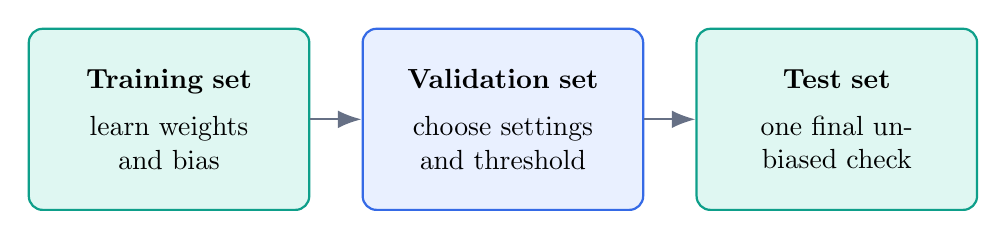
\begin{tikzpicture}[node distance=.65cm]
      \node[data,text width=3cm,minimum height=2.3cm](train){\textbf{Training set}\\[5pt]learn weights and bias};
      \node[box,text width=3cm,minimum height=2.3cm,right=of train](val){\textbf{Validation set}\\[5pt]choose settings and threshold};
      \node[data,text width=3cm,minimum height=2.3cm,right=of val](test){\textbf{Test set}\\[5pt]one final unbiased check};
      \draw[flow](train)--(val);\draw[flow](val)--(test);
    \end{tikzpicture}
  \end{center}
  \vspace{.7cm}\takeaway{Every time a test result changes what we do, the test quietly becomes training data.}
\end{frame}

\begin{frame}{This loop leaks information}
  \begin{center}
    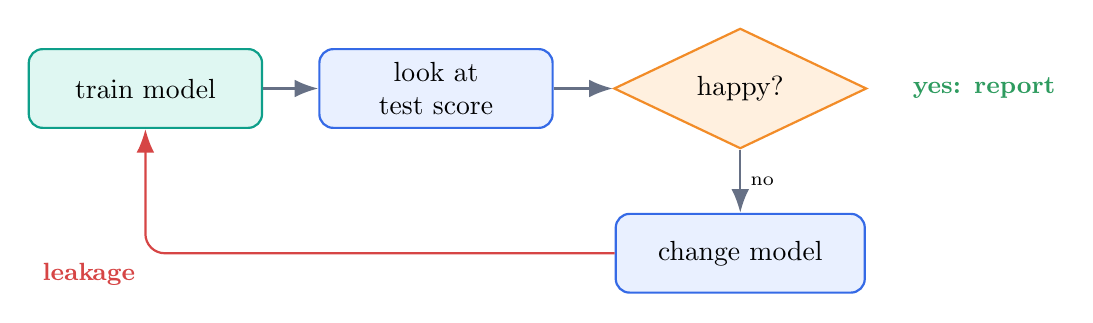
\begin{tikzpicture}[node distance=.7cm]
      \node[data,text width=2.4cm](train){train model};
      \node[box,text width=2.4cm,right=of train](test){look at test score};
      \node[decision,right=.75cm of test,text width=1.9cm](happy){happy?};
      \node[box,below=.8cm of happy,text width=2.6cm](tune){change model};
      \draw[flow](train)--(test);\draw[flow](test)--(happy);
      \draw[flow](happy)--node[right,font=\scriptsize]{no}(tune);
      \draw[flow,Red,rounded corners=7pt](tune.west)-|node[below left,font=\small\bfseries,text=Red]{leakage}(train.south);
      \node[Green,right=.45cm of happy,font=\small\bfseries]{yes: report};
    \end{tikzpicture}
  \end{center}
  \vspace{.45cm}\question{If we try 20 models and report the best test score, is the test still untouched?}
\end{frame}

\begin{frame}{Cross-validation makes better use of limited data}
  \begin{center}
    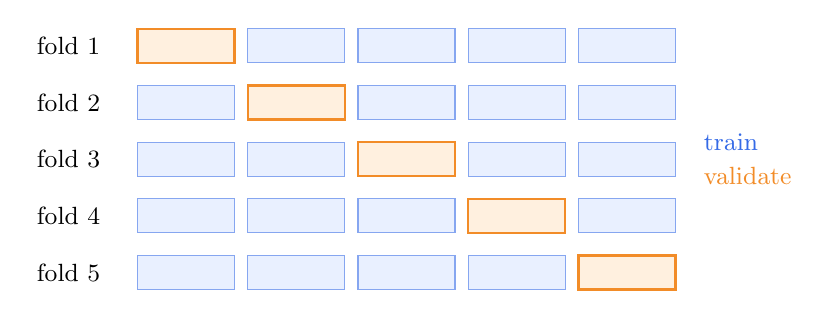
\begin{tikzpicture}[x=1.4cm,y=.72cm]
      \foreach \r in {0,...,4}{
        \pgfmathtruncatemacro{\fold}{\r+1}
        \node[anchor=east,font=\small]at(-.25,-\r){fold \fold};
        \foreach \c in {0,...,4}{
          \ifnum\r=\c\fill[OrangeLight,draw=Orange,thick](\c,-\r-.3)rectangle++(.88,.6);
          \else\fill[BlueLight,draw=Blue!60](\c,-\r-.3)rectangle++(.88,.6);\fi}}
      \node[anchor=west,font=\small,text=Blue]at(5.05,-1.7){train};
      \node[anchor=west,font=\small,text=Orange]at(5.05,-2.3){validate};
    \end{tikzpicture}
  \end{center}
  \vspace{.3cm}
  \begin{itemize}
    \item Each fold gets one turn as validation data
    \item Average scores to compare model choices
    \item Inspect the spread to understand stability
    \item Keep the final test set outside the entire process
  \end{itemize}
\end{frame}

\begin{frame}{The honest workflow}
  \begin{center}
    \resizebox{.96\textwidth}{!}{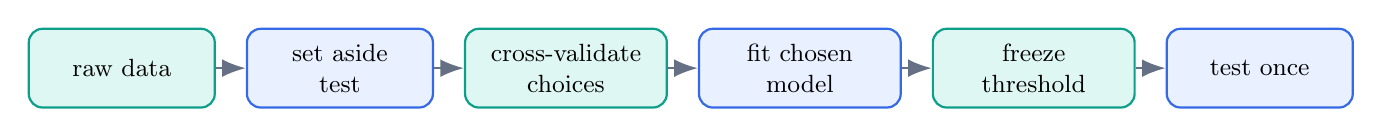
\begin{tikzpicture}[node distance=.38cm,every node/.style={font=\small}]
      \node[data,text width=1.8cm](raw){raw data};
      \node[box,text width=1.8cm,right=of raw](split){set aside test};
      \node[data,text width=2cm,right=of split](cv){cross-validate choices};
      \node[box,text width=2cm,right=of cv](fit){fit chosen model};
      \node[data,text width=2cm,right=of fit](freeze){freeze threshold};
      \node[box,text width=1.8cm,right=of freeze](final){test once};
      \draw[flow](raw)--(split);\draw[flow](split)--(cv);\draw[flow](cv)--(fit);\draw[flow](fit)--(freeze);\draw[flow](freeze)--(final);
    \end{tikzpicture}}
  \end{center}
  \vspace{.65cm}
  \begin{itemize}
    \item Fit preprocessing on training folds only
    \item Choose learning rate, features, and threshold without the test set
    \item Report the final metric and the cost of each kind of mistake
  \end{itemize}
\end{frame}

% ================================================================
% Wrap-up: summarize concepts, then connect to the exercise once
% ================================================================
\section{Wrap-up}

\begin{frame}{The logic of the lecture}
  \begin{center}
    \resizebox{.96\textwidth}{!}{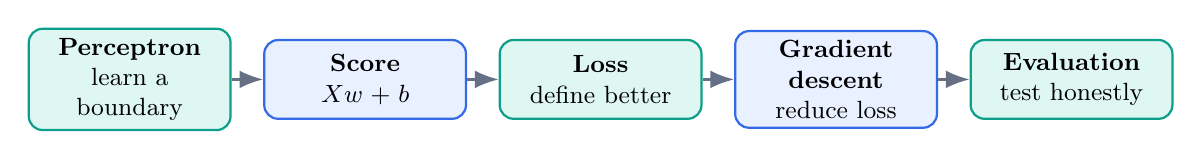
\begin{tikzpicture}[node distance=.4cm,every node/.style={font=\small}]
      \node[data,text width=2cm](p){\textbf{Perceptron}\\learn a boundary};
      \node[box,text width=2cm,right=of p](s){\textbf{Score}\\$Xw+b$};
      \node[data,text width=2cm,right=of s](l){\textbf{Loss}\\define better};
      \node[box,text width=2cm,right=of l](g){\textbf{Gradient descent}\\reduce loss};
      \node[data,text width=2cm,right=of g](e){\textbf{Evaluation}\\test honestly};
      \draw[flow](p)--(s);\draw[flow](s)--(l);\draw[flow](l)--(g);\draw[flow](g)--(e);
    \end{tikzpicture}}
  \end{center}
  \vspace{.65cm}
  \begin{itemize}
    \item Linear and logistic regression reuse the perceptron's weighted score
    \item Activation determines the output; loss determines learning
    \item A useful model needs both good predictions and honest evaluation
  \end{itemize}
\end{frame}

\appendix
\begin{frame}{Reference: model and loss formulas}
  \begin{align*}
    \text{Weighted score:}\quad&z=Xw+b\\[4pt]
    \text{Linear prediction:}\quad&\hat y=z\\[4pt]
    \text{Logistic probability:}\quad&p=\frac{1}{1+e^{-z}}\\[4pt]
    \text{MSE:}\quad&\text{average}\big((\hat y-y)^2\big)\\[4pt]
    \text{BCE:}\quad&-\text{average}\big(y\log p+(1-y)\log(1-p)\big)
  \end{align*}
\end{frame}

\begin{frame}{Reference: metric formulas}
  \begin{columns}[T,onlytextwidth]
    \column{.47\textwidth}\begin{align*}
      \text{Accuracy}&=\frac{TP+TN}{TP+TN+FP+FN}\\[5pt]
      \text{Precision}&=\frac{TP}{TP+FP}\\[5pt]
      \text{Recall}&=\frac{TP}{TP+FN}
    \end{align*}
    \column{.47\textwidth}\begin{align*}
      F_1&=\frac{2PR}{P+R}\\[5pt]
      F_2&=\frac{5PR}{4P+R}
    \end{align*}
  \end{columns}
\end{frame}

\end{document}





